\chapter{Grandezas Proporcionais}

\section{Introdução}

\quad O conceito de proporção tem uma importância muito grande, não apenas em matemática como também no cotidiano. Frequentemente, empregamos proporções em nosso dia-a-dia, embora sem utilizar símbolos matemáticos. 

\quad Quando fazemos uma justa crítica de uma estátua, dizendo que "ela tem uma cabeça muito grande", não estamos nos referindo à medida absoluta da cabeça. Em uma estátua, a cabeça pode ser $``$muito grande$"$ , mesmo medindo a metade, um quarto ou um décimo da cabeça verdadeira; é $``$muito grande$"$  \textbf{proporcionalmente }ao conjunto da própria estátua.

O conceito de proporções está presente em vários temas da vida cotidiana e da ciência, como por exemplo: porcentagem, juros simples, triângulos semelhantes, espaço e tempo em um deslocamento com velocidade constante, receitas culinárias, relação entre custo e quantidade de produtos produzidos ou consumidos, consumo de combustível, composição de combustíveis, escala de mapas, além de tantos outros temas.


\section{Razões}
 
\begin{caixa}
\begin{tdefinicao}
	Dados dois números racionais \textit{a} e \textit{b}, com \textit{b $\neq$ 0}, chama-se razão entre \textit{a} e \textit{b} ao quociente indicado $\frac{a}{b}$ por ou $a \, : \, b$,
	onde \textit{a} é 1º termo ou \textit{antecedente} e \textit{b }é o 2º termo ou \textit{consequente}.
\end{tdefinicao}
\end{caixa}

\begin{texemplo} 
Em uma sala de aula existem 25 homens e 20 mulheres.

\begin{enumerate}[label=\arabic*]
	\item Determine a razão do número de mulheres para o número de homens desta turma.

	\item Determine uma razão equivalente à razão do item anterior.

	\item Encontre a razão do número de homens para o número de mulheres desta turma.

	\item Determine uma razão equivalente à razão do item anterior.\quad 
\end{enumerate}


\textbf{Solução}: a) Pela Def. 2.1: 

$$r=\frac{20}{25} $$

b) Uma razão equivalente à razão \textit{r} é  \( r=\frac{20}{25}=\frac{4}{5} \)  .

c) A razão do número de homens para o número de mulheres é\   \( p=\frac{25}{20} \) .

d) Uma razão equivalente à razão dada é  \( p=\frac{25}{20}=\frac{5}{4} \)  \qedsymbol{}

\end{texemplo}
Muitos conceitos importantes são expressos por razões:

\begin{texemplo} 
	Na elaboração de vinhos o rendimento é a razão entre a quantidade de vinho produzida pela massa de uva utilizada. Se \textit{2000 l} de vinho foram produzidos com \textit{2400 kg} de uvas, qual foi o rendimento :
	
\textbf{Solução}:\ O rendimento é uma razão:   \( r=\frac{2000}{2600}=0,769 \) \qedsymbol{}
\end{texemplo}

\textbf{Densidade demográfica}: razão entre o número de habitantes de uma região e a área dessa região.
\begin{caixa}
	Densidade demográfica = $\dfrac{habitantes}{area}$
\end{caixa}

\textbf{Densidade de um corpo}: razão entre a massa de um corpo e o seu volume.
\begin{caixa}
	Densidade = $\dfrac{massa}{volume}$
\end{caixa}

\textbf{Velocidade média}: razão entre a distância percorrida por um móvel e o tempo gasto para percorrê-la.
\begin{caixa}
	Velocidade media = $\dfrac{\textrm{distância}}{tempo}$
\end{caixa}

\textbf{Escala}: razão entre a medida de um comprimento no desenho e a medida correspondente ao comprimento real.
\begin{caixa}
	Escala = $\dfrac{medida\,do\,comprimento\,do\,desenho}{medida\,do\,comprimento\,real}$
\end{caixa}

\textbf{Porcentagem}: razão entre um número natural e cem.
\begin{caixa}
	Porcentagem = $\dfrac{\textrm{número natural}}{100}$
\end{caixa}

\begin{texemplo}
	No vestibular inscreveram-se 7830 candidatos para disputarem as 90 vagas de um curso. Qual a relação candidato-vaga para esse curso?

	\textbf{Solução: }Usando a Def. 1.1, vamos expressar a relação candidato-vaga como uma razão:

	\( \frac{7830}{90}=\frac{87}{1} \)  . Isto significa que existem 87 candidatos para 1 vaga \qedsymbol{}
\end{texemplo}
\begin{texemplo}
	Uma solução A contém 279 litros de álcool e 1116 litros de água e, a solução B, contém 1155 litros de álcool e 5775 litros de água. Qual das duas soluções tem maior teor alcóolico?

	\textbf{Solução: }Escrevendo as razões das duas soluções e efetuando a divisão, temos os teores de álcool

	\( \frac{279}{1116}=0,25 \) \ \ \ \ \ \  \quad e \quad \quad   \( \frac{1155}{5775}=0,2 \) 

	Assim, a solução A temo maior teor de álcool \qedsymbol{}
\end{texemplo}
\begin{texemplo}
	A razão entre $\frac{5}{2}$ e $\frac{3}{10}$ é?

\textbf{Solução:} A razão entre os dois números é \( \frac{\frac{2}{5}}{\frac{3}{10}}=\frac{2}{5} \cdot \frac{10}{3}=\frac{4}{3} \) \qedsymbol{}

\end{texemplo}

\begin{exercicios}

	\exitem{} Determine a razão entre os números abaixo:

\begin{multicols}{4}
	a)$3$ e $\frac{6}{7}$
	
	b)$\frac{1}{2}$ e $\frac{1}{3}$
	
	c)$1,5$ e $5$
	
	d)$7$ e $3 \frac{2}{4}$
\end{multicols}

	\exitem{} A massa A é 10 kg e massa B é 5.000g. Qual a razão entre as massas A e B ?

	\exitem{} Numa razão igual a $\frac{2}{5}$ o antecedente é 8. Determine a razão.

	\exitem{} O triplo do consequente de uma razão igual a é 63. Determine o antecedente e a razão inversa.

	\exitem{} Num jogo de basquete, André fez 60 arremessos, obtendo 50 pontos e Paulo, em 30 arremessos, obteve 20 pontos. Quem obteve a maior razão de acerto?

	\exitem{} O perímetro de um triângulo é 28m e o lado de um quadrado mede 9m. Qual é a razão entre os perímetros?

\end{exercicios}

\section{Proporções e Regra de Três }

\quad Em certas situações práticas do cotidiano, somos levados a ter de escolher entre duas ofertas, verificando qual é a mais econômica. Por exemplo, na compra de 2 potes de manteiga da mesma marca, um com 300g custa R\$  1,50 o outro com 1000g custa R\$ 4,80. Fazendo as razões das duas opções, obtemos 200 R\$ /g e 208,33 R\$ /g, respectivamente. Como vemos o primeiro pote é o mais barato. Neste caso, dizemos que as razões de preço por massa não estão \textit{proporcionais}. 

\begin{caixa}
	\begin{tdefinicao}
		Sejam\   \( \frac{a}{b} \) \ \ \ e   \( \frac{c}{d} \) \ \  duas razões, com \textit{b $ \neq $  0} e \textit{c $ \neq $  0}. Uma \textit{proporção} é a igualdade entre duas razões.

		$$ \frac{a}{b}=\frac{d}{c} $$

		Onde \textit{b} e \textit{d} são os meios e \textit{a} e \textit{c} são os extremos.
	\end{tdefinicao}
\end{caixa}
Lê-se: \textit{a} está para \textit{b} assim como \textit{c} está para \textit{d} e escreve-se, alternativamente, \textit{a : b :: c : d}.

\subsection{Propriedade fundamental das proporções:}

Em toda a proporção, o produto dos meios é igual ao produto dos extremos, ou seja:

$$\dfrac{a}{b}=\dfrac{c}{d} \textrm{ então } bc \, = \, ad$$
\begin{FlushRight}
(3.1)
\end{FlushRight}

\subsection{Outras propriedades das proporções:}

\textbf{P1:} $\dfrac{a}{b}=\dfrac{c}{d} \Longleftrightarrow \dfrac{a+b}{a}=\dfrac{c+d}{c}$

\textbf{P2:} $\dfrac{a}{b}=\dfrac{c}{d} \Longleftrightarrow \dfrac{a+b}{b}=\dfrac{c+d}{d}$

\textbf{P3:} $\dfrac{a}{b}=\dfrac{c}{d} \Longleftrightarrow \dfrac{a-b}{a}=\dfrac{c-d}{c}$

\textbf{P4:} $\dfrac{a}{b}=\dfrac{c}{d} \Longleftrightarrow \dfrac{a-b}{b}=\dfrac{c-d}{d}$

\textbf{P5:} $\dfrac{a}{b}=\dfrac{c}{d} \Longleftrightarrow \dfrac{a+c}{b+d}=\dfrac{a}{b}\,$ e $\,\dfrac{a+c}{b+d}=\dfrac{c}{d}$

\textbf{P6:} $\dfrac{a}{b}=\dfrac{c}{d} \Longleftrightarrow \dfrac{a-c}{b+d}=\dfrac{a}{b}\,$ e $\,\dfrac{a-c}{b+d}=\dfrac{c}{d}$

\textbf{P7:} $\dfrac{a}{b}=\dfrac{c}{d} \Longleftrightarrow \dfrac{b}{a}=\dfrac{d}{c}$

\begin{texemplo}
	Calcular o valor de x na proporção:

	\textbf{Solução: }Usando a propriedade fundamental das proporções, temos:

	\textit{3 $ \cdot $  20 = 5 $ \cdot $  (x + 1)}

	\textit{60 = 5x + 5}

	\textit{x = 11}\qedsymbol{}
\end{texemplo}

\begin{texemplo}
	Em uma equipe olímpica, 25 atletas são rapazes. Qual é o número de moças, se a razão entre o número de rapazes e moças é cinco terços.

	\textbf{Solução:} Sendo \textit{x o número de moças e escrevendo os dados do problema como uma proporção, temos:}

	\[ \frac{25}{x}=\frac{5}{3} \] 

	\quad Usando a propriedade fundamental das proporções temos 

	\textit{5 $ \cdot $  x = 3 $ \cdot $  25 }

	\textit{x =15 }moças\textit{ }\qedsymbol{}
\end{texemplo}

\begin{exercicios}

	\exitem{} Calcule o valor de x nas proporções:
	\begin{multicols}{4}
		a) $\dfrac{2}{5}=\dfrac{x}{6,25}$
		
		b) $\dfrac{1-\frac{1}{3}}{0,5}=\dfrac{4}{x}$
		
		c) $\dfrac{x}{3 - 0,75}=\dfrac{4}{2-\frac{1}{8}}$
		
		d) $\dfrac{3}{2 - \frac{3}{4}}=\dfrac{2 + \frac{3}{4}}{x}$
	\end{multicols}

	\exitem{} Uma vara de 12cm fixada verticalmente no solo produz uma sombra de 15cm. Que comprimento deveria ter a vara para projetar uma sombra de 45cm?

	\exitem{} Uma foto de dimensões 3cm x 4cm foi ampliada passando o seu comprimento de 4cm para 28cm. Quanto passou a medir a sua largura?

	\exitem{} A soma dos perímetros de dois quadrados é 52cm. Determine esses perímetros sabendo que a razão entre eles é de $\frac{3}{10}$.

	\exitem{} Dividiu-se 14kg de carne entre duas pessoas, sendo a razão entre as partes igual a $\frac{3}{4}$. Quanto recebeu cada pessoa? 

	\exitem{} A idade de um pai e a de seu filho estão na razão $\frac{3}{1}$. Qual a idade de cada um, sabendo que a diferença entre elas é de 24 anos?

	\exitem{} A diferença entre os comprimentos de duas peças de fazenda é de 15m e estão entre si como 7 está para 4. Calcule a metragem de cada peça.

	\exitem{} Um pai tem 36 anos e sua idade é $\frac{4}{5}$ da soma das idades de seus dois filhos. Quais as idades dos filhos, sabendo-se que elas estão entre si como 4 esta para 5?

	\exitem{} Calcule x e y na proporção $\frac{x}{4}=\frac{y}{8}$, sabendo que $5x+3y=33$

	\exitem{} Calcule a e b na proporção $\frac{a}{3}=\frac{b}{6}$ , sabendo que $5a-2b=2$

	\exitem{} Calcule a, b e c em $\frac{a}{7}=\frac{b}{14}=\frac{c}{21}$, sabendo que $2a-b+2c=12$

	\exitem{} Calcule b nas igualdades $\frac{3}{a}=\frac{6}{b}=\frac{12}{c}=\frac{15}{d}$, sabendo que $3a+c+2d=85$

	\exitem{} Calcule a e b na proporção $\frac{a}{7}=\frac{b}{14}$, sabendo que $a^2+b^2=20$

	\exitem{} Calcule a e b na proporção $\frac{3}{a}\frac{6}{b}$, sabendo que $5a^2-b^2=64$

	\exitem{} Dividir o número 570 em três partes tais que a primeira esteja para a segunda como 4 esta para 5 e a segunda esteja para a terceira como 6 esta para 12. Nestas condições, a terceira parte vale...

	\exitem{} Divida 305 em três partes tais que a primeira esteja para a segunda como 2 esta para 5 e a segunda esteja para a terceira como 3 esta para 8. 

	\exitem{}  Dois líquidos A e B estão misturados em um volume total de 56 litros, na razão de 9 para 5. Calcular o volume de cada substância. 

	\exitem{} O salário de duas pessoas estão entre si, assim como 11 está para 14. Calcular esses salários sabendo que o triplo do salário do primeiro menos o dobro do salário do segundo é R\$  150,00. 

	\exitem{}  Dividir o lucro de R\$ 2.500,00 entre três pessoas de modo que a 2ª receba dois quintos da 1ª e a 3ª receba três meios da 2ª.

	\exitem{}  Sabe-se que a razão entre o número de médicos e o número de habitantes de uma cidade é de $\frac{1}{2500}$. Se há 30 médicos nessa cidade, qual é a sua população?

	\exitem O número de meninos e o número de meninas estão na razão de 3 para 4, quantos são os meninos, se as meninas são em número de 52?

\end{exercicios}

\section{Regras de sociedade }

\quad A regra de sociedade é uma das aplicações da divisão proporcional. Tem por objeto a divisão dos lucros ou dos prejuízos entre as pessoas (sócios) que formam uma sociedade, por ocasião do balanço geral exigido anualmente por lei ou, quando da saída de um dos sócios ou, da admissão de um novo sócio. 


\quad Por convenção o lucro ou prejuízo é dividido pelos sócios proporcionalmente aos capitais que empregaram, levando-se em conta as condições estipuladas no contrato social.

\quad Classicamente, há dois tipos a considerar: Regra de sociedade simples e composta.

\quad \textbf{Regra de Sociedade Simples }

\begin{enumerate}[label=\arabic*)]
	\item Quando os capitais são diferentes e os tempos são iguais

	\item Quando os capitais são iguais e os tempos são diferentes. 
\end{enumerate}

Ambos os casos são resolvidos usando conhecimentos de divisão em partes proporcionais. 

\begin{texemplo}
	Antônio, José e Pedro se associaram para comprar um terreno no valor de R\$  60.000,00. Antônio entrou com R\$  30.000,00, José com R\$  20.000,00 e Pedro com R\$ 10.000,00. Algum tempo depois venderam o terreno por R\$ 90.000,00. Qual a parte que coube a cada um deles?


\textbf{Solução: }A cada real empregado na compra do terreno deve corresponder a mesma quantia resultante da venda, isto é, uma quota. Essa quota é, na verdade, o quociente do preço de venda pelo preço da compra, ou seja:

$\dfrac{P\text{\textsubscript{v}}}{P\text{\textsubscript{c}}}=\dfrac{90.000}{60.000}=1,5$\quad  (coeficiente de proporcionalidade)

Os três sócios devem receber as seguintes quantias:

	Antônio: $R\$30.000,00 \times 1,5 = R\$45.000,00$ 

	José: $R\$20.000,00 \times 1,5 = R\$30.000,00$

	Pedro: $R\$10.000,00 \times 1,5 = R\$15.000,00$

Escrevendo as razões entre as quantias recebidas e empregadas individualmente, observamos que as quantias que os sócios receberam na venda são números proporcionais às quantias empregadas na compra do terreno.

$$\dfrac{45.000}{30.000}=\dfrac{30.000}{20.000}=\dfrac{15.000}{10.000}=1,5 \textrm{\qedsymbol{}}$$
\end{texemplo}

\quad \textbf{Regra de Sociedade Composta}

\quad Neste caso tanto os capitais quanto os períodos de tempo são diferentes para cada sócio. Então os lucros ou prejuízos serão divididos em partes diretamente proporcionais ao produto dos capitais pelos respectivos períodos de tempo.

\begin{texemplo}
	Numa sociedade, após um ano de atividades o lucro foi de R\$  46.739,34. O segundo sócio entrou na sociedade após 3 meses do funcionamento com o capital de R\$ 7.580,00. Se o capital do primeiro sócio é de R\$ 6.920,00, determine a parte de cada sócio nesse lucro.

	\textbf{Solução: }Participação do 1º sócio (A) – 12 meses – capital\  - R\$ 6.920,00 x 12 meses = R\$  83.040,00

	Participação do 2º sócio(B)\ – 9 meses – capital  - R\$  7.580,00 x 9 meses = R\$  68.220,00
	$$\frac{A}{83.040} = \frac{B}{68.220} = \frac{A+B}{83.040+68220} = \frac{46.739,34}{151.260} = 0,309$$

	$\frac{A}{83.040} = 0,309 \longrightarrow A = 25.659,36$; $\frac{B}{68.220} = 0,309 \longrightarrow B = 21.079,98$ \qedsymbol{}
\begin{flushright}
	(P5)
\end{flushright}
\end{texemplo}
\begin{exercicios}

	\exitem{} O capital social de uma empresa é formado na razão de dois terços. Determine a parte de cada sócio no lucro líquido de R\$ 11.360,00, apurado no último balanço.

	\exitem{} Uma empresa com três sócios tem seu capital constituído da seguinte forma: o primeiro sócio tem R\$  2.380,00; o segundo tem 20\% a mais que o primeiro e o terceiro tem a metade do segundo. Se o lucro dessa empresa no último balanço foi de  R\$ 19.600,00 dos quais 21,8\%  corresponde as despesas. Determine qual a parte de cada sócio no lucro líquido dessa empresa.

	\exitem{} Dois sócios\  montaram uma empresa com 50\%  do capital social financiado em um banco com taxa de mercado. Após sete meses de funcionamento, com dificuldades financeiras, admitiram um terceiro sócio. No fim de um ano, a empresa apresentou um lucro líquido de R\$  2.407,00, sendo integralizado no capital da empresa. Qual a parte de cada sócio nesse lucro? 

	\exitem{} A razão entre os capitais de dois sócios numa empresa é de três quintos. Se o sócio A recebeu R\$ 3.255,00 de lucro, calcule o lucro do sócio B.

	\exitem{} A importância de R\$  1.085,00 foi dividida entre três pessoas. Sabendo-se que a parte da primeira está para a segunda como sete está para nove e que a parte da segunda está para a terceira assim como três está para cinco, determine essas partes.

	\exitem{} Numa empresa o prêmio de R\$  1.000,00 será dividido entre os dois funcionários com maior produtividade. Sabendo que os classificados têm 80 e 120 pontos, quanto cada um vai receber?

	\exitem{} O lucro de uma indústria foi dividido entre três sócios na proporção de 6, 10 e 18. Sabendo que o segundo sócio recebeu R\$  4.000,00 a mais que o primeiro, pergunta-se: 

	a) Qual foi o lucro total? 

	b) Quanto cada sócio recebeu?

	\exitem{}  Uma empresa teve um lucro de R\$  25.000,00, dos quais, quatro quintos serão divididos entre seus dois sócios, proporcionalmente aos capitais investidos na formação do capital social dessa empresa. Se o primeiro sócio participou com R\$  4.000,00 e o segundo com R\$  6.000,00; quanto cada um vai receber desse lucro?

	\exitem{} Em uma empresa 40\% do lucro será aplicado na compra de equipamentos e um quarto, também desse lucro, que corresponde à R\$ 5.000,00 será destinado para a manutenção das instalações. O restante será dividido entre os sócios de acordo com o capital de cada um nessa sociedade. Se os capitais investidos foram: R\$  3.000,00; R\$  4.000,00 e R\$  7.000,00, calcule quanto cada sócio vai receber e quantos reais foram aplicados em equipamentos? 

	\exitem{} Ao dividir um número em partes diretamente proporcionais aos números 4, 3 e 5, achou-se que a parte correspondente ao número 3 era\ 150. Determine esse número.  

	\exitem{} As cotas de participação no capital social de uma empresa, variam de acordo com o capital de cada sócio na formação desse capital. A razão entre os capitais dos sócios C e D é de dois terços e juntos somam quatro quintos do capital E. Calcule o capital C e D sabendo que o capital E é de R\$  9.000,00. 

\end{exercicios}

\section{Grandezas Diretamente e Inversamente Proporcionais}

Considere um quadrado de lado $l$ e perímetro P. A razão entre P e $l$ é 4, pois P = 4. Além disso, isto significa que P e $l$ são variáveis diretamente proporcionais pois, quando uma aumenta (ou diminui), a outra também aumenta (ou diminui).

No caso de um retângulo de largura $l$, altura h e área de 36$m^2$, ocorre algo diferente:  $l$ e h são variáveis inversamente proporcionais, já que l $ \cdot $  h = 36. Neste caso, quando uma aumenta a outra diminui e, vice-versa.

\subsection{Regra de três}

\quad Caso três termos sejam conhecidos na proporção, podemos calcular o quarto. Essa relação é o que conhecemos por \textit{Regra de Três. }Ou ainda, é um modo prático de encontrar um termo desconhecido, dados outros 3. 

\subsubsection{Regra de Três direta e Regra de Três inversa}
\quad Observe as situações:

\begin{enumerate}[label=(\roman*)]
	\item Um restaurante prepara 500 refeições por dia. Quantas refeições terá preparado no final de um mês, considerando 20 dias úteis de trabalho?

	\item Para pintar uma casa em nove dias é necessário um pintor. Quantos pintores serão necessários para executar o mesmo serviço em 3 dias?

	\item  Ana tem 2 anos e 90 cm de altura. Qual será a altura de Ana aos 6 anos?
\end{enumerate}

Na situação (i) aumentando-se uma das grandezas a outra também aumenta na mesma razão, ou então, diminuindo-se uma das grandezas a outra também diminui na mesma razão, temos assim \textit{grandezas diretamente proporcionais.}

Na situação (ii), ocorre o inverso, aumentando-se uma das grandezas a outra diminui na razão inversa, ou então, diminuindo-se uma das grandezas a outra aumenta na razão inversa, temos assim \textit{grandezas inversamente proporcionais}.

Veja que na situação (iii) uma grandeza aumenta e a outra também aumenta, mas \textit{não são proporcionais} (nem direta, nem inversamente), pois a razão de variação das grandezas é diferente, não sendo possível calcular por Regra de Três.


\subsubsection{Resolução de Regra de Três}
	Para resolver uma Regra de Três sugere-se seguir os seguintes passos:

1º) montar um proporção com a indicação das grandezas envolvidas e os valores de cada uma;

2º) verificar se as grandezas envolvidas são direta ou inversamente proporcionais;

3º) montar uma proporção envolvendo os valores das grandezas. Se as grandezas forem inversamente proporcionais devemos inverter uma das razões antes de formar a proporção e calcular o termo desconhecido.

\begin{texemplo}
Em  50ml de gasolina, 10 ml é álcool. Quantos litros de álcool contém uma amostra de  20$l$ de gasolina?

50ml de gasolina \quad \quad \quad \quad 10 ml álcool

20$l$ de gasolina \quad \quad \quad \quad x (variável)

\textbf{Solução:} Inicialmente, neste caso, é necessário transformar as unidades: 20$l$ = 20000 ml. Escrevendo a regra de três como uma proporção, temos:
$\dfrac{50}{20000}=\dfrac{10}{x}$ 

As grandezas são diretamente proporcionais, pois se aumentar o volume da solução aumenta também o volume de álcool. 
Usando a propriedade fundamental das proporções e resolvendo para x, temos x = 4 000 ml  ou 4$l$  de álcool \qedsymbol{}
\end{texemplo}

\begin{texemplo}

	Para pintar uma casa em nove dias é necessário um pintor. Quantos pintores serão necessários para executar a mesma casa em 3 dias?
	\textbf{Solução:} Escrevendo a regra de três como uma proporção, temos 
	$$\uparrow \dfrac{9}{1} = \dfrac{3}{x} \downarrow$$
	As grandezas são inversamente proporcionais, pois quanto mais pintores trabalharem, menos dias serão necessários. Invertendo a segunda razão, temos:
	$$\dfrac{9}{1} = \dfrac{x}{3}$$ 
 
	Usando a propriedade fundamental das proporções e resolvendo para x, temos x = 27 pintores para pintar a casa em 3 dias \qedsymbol{}

\end{texemplo}

\subsubsection{Regra de Três Composta}
	Quando queremos calcular um valor desconhecido e são envolvidas mais de duas grandezas podemos utilizar uma Regra de Três Composta. 

	Para resolvê-la, sugere-se os seguintes passos: \linebreak
	1º) Verificar se as grandezas envolvidas são direta ou inversamente proporcionais, analisando cada grandeza com a que possui o termo desconhecido, desconsiderando as outras. Lembrar que que quando a grandeza for inversamente proporcional, devemos inverter a razão ao formar a proporção.

	2º) construir uma proporção entre as grandezas igualando a razão que possui o termo desconhecido com o produto de todas as outras razões envolvidas no problema. \linebreak
	3º) Resolver a proporção usando as propriedades de proporções.

\begin{texemplo}

	Quatro operários produzem, em 10 dias, 320 peças de certo produto. Quantas peças desse mesmo produto serão produzidas por 10 operários em 16 dias?
	\textbf{Solução:} Seguindo os passos sugeridos, observamos que o termo desconhecido é o número de peças. Este número aumenta na medida em que aumenta o número de operários e o número de dias trabalhados, portanto as três grandezas são diretamente proporcionais.

\begin{figure}[H]
	\begin{center}
		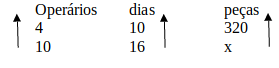
\includegraphics{capitulos/grandezas_proporcionais/media/image08.png}
	\end{center}
\end{figure}

Construindo a proporção, temos:
$$\dfrac{4}{10} \cdot \dfrac{10}{16}=\dfrac{320}{x}$$

Resolvendo para x, obtemos  x = 1280 peças \qedsymbol{}
\end{texemplo}

\begin{texemplo} 
	Se 10 trabalhadores constroem uma ponte em 12 dias, em quantos dias 8 trabalhadores construiriam essa mesma ponte?
	\textbf{Solução:}  Seguindo os passos sugeridos, observamos que o termo desconhecido é o número de dias necessários para construir a ponte, que é inversamente proporcional ao número de trabalhadores.  
	\begin{figure}[H]
		\begin{center}
			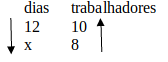
\includegraphics{capitulos/grandezas_proporcionais/media/image09.png}
		\end{center}
	\end{figure}

	Construindo a proporção, temos: $\dfrac{12}{x}=\dfrac{8}{10}$
	Resolvendo para x, obtemos  x = 15 dias \qedsymbol{}
\end{texemplo}

\begin{texemplo} 

Uma firma construtora preparou 20 km de leito da estrada contratada em 200 dias e 8 horas de jornada de trabalho, utilizando-se 9 máquinas e empregando 45 homens. Em quantos dias de trabalho, concluirá a preparação de outros 24 km, da mesma estrada, se utilizar na obra 10 máquinas e 48 homens em jornada diária de 9 horas, sabendo-se que a dificuldade deste trecho é $\frac{4}{5}$do trecho concluído?    

\textbf{Solução:} Seguindo os passos sugeridos, observamos que o termo desconhecido é o número de dias trabalhados. Os dias trabalhados são diretamente proporcionais a quilometragem e à dificuldade da obra, porém inversamente proporcional à jornada de trabalho, ao número de máquinas e de operários. 
\begin{figure}[H]
	\begin{center}
		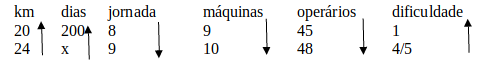
\includegraphics{capitulos/grandezas_proporcionais/media/image10.png}
	\end{center}
\end{figure}

Construindo a proporção, temos:
$$\dfrac{200}{x}=\dfrac{20}{24}\cdot \dfrac{9}{8}\cdot \dfrac{10}{9} \cdot \dfrac{48}{45} \cdot \dfrac{1}{4/5}$$
Resolvendo para x, obtemos  x = 144 dias  \qedsymbol{}
\end{texemplo}

\begin{exercicios}
	\exitem{} Um carro faz, na estrada 8 km com um litro de álcool.

		a) quantos litros de álcool são necessários para esse carro percorrer 100 km?

		b) quantos km ele percorre com 45 litros de álcool?
	\exitem{} A secretária de um empresa  preenche 10 fichas de cadastro de clientes  em 30 minutos.

		a) quanto tempo ele leva para preencher o cadastro de  50 clientes?

		b) quantos cadastros  ela  preenche em 2 horas de trabalho interruptas?
	\exitem{} Um relógio atrasa 2 minutos a cada 24 horas.

		a) quantos minutos atrasará em 60 horas?
	
		b) quantos minutos atrasará em 15 dias?
	
		c) depois de quantos dias ele ficará 20 minutos atrasados?	
	\exitem{} Com 3,5 litros de tinta, Antonio pinta uma parede com 14m$^2$. 
	
	a) que superfície ele pode pintar com 18 litros de tinta?			
	
	b) qual o volume de tinta necessário para pintar uma pintar uma parede de 36m$^2$ ?
	\exitem{} Numa fazenda, cada boi come a mesma quantidade de ração todos os dias. O fazendeiro, que tinha armazenado ração suficiente para alimentar seus 40 bois durante 25 dias, comprou mais 10 bois. Nesse caso, quantos dias a ração deve durar?		
	\exitem{} Um corredor de fórmula I dá uma volta na pista em um minuto e 30 segundos, a uma média de 200km/h. 
	
	a) em quanto tempo fará a volta na pista, se mantiver a velocidade média de 180km/h?	
	
	b) para fazer a volta em 1minuto e 15 segundos, qual deve ser a sua velocidade média?	
	\exitem{} Uma equipe de 8 pessoas leva 10 dias para pintar um casa. Quanto tempo levaria uma equipe de 20 pessoas?				
	\exitem{} Para pintar uma parede de 9 metros de comprimento por 3 metros de altura, foi gasto uma lata de tinta. Usando uma lata de tinta igual, quantos metros do comprimento da parede posso pintar, se ele tiver 1,8 metros de altura.	
	\exitem{} Com 100kg de trigo pode-se fazer 85 kg de farinha. Qual a quantidade de farinha que se obtém com 480 kg de trigo?
	\exitem{} A sombra de uma chaminé mede 4,5m e a de uma vara vertical, no mesmo instante, é 0,9m.  Calcule a altura da chaminé sabendo-se que a vara tem 2m de comprimento.         
	\exitem{} Um parafuso avança 33mm em cada 6 voltas. Qual o número de voltas apara avançar 77mm?  
	\exitem{} Uma torneira despeja em meia hora 600 litros de água. Quantos litros são escoados em 8 minutos?                
	\exitem{} Em cada 3m$^2$ de uma fazenda são plantadas 15 sementes. O número de hectares necessários para se plantar 200 mil sementes é...
	\exitem{} Uma roda com 50 dentes engrena com outra de 40. Qual o número de voltas da primeira, quando a segunda dá 600 voltas por minuto?                                                                                               
	\exitem{} Uma pessoa x pode realizar uma certa tarefa em 12 horas. A outra pessoa y, é 50\% mais eficiente que x. Nessas condições, o número de horas necessárias para que y realize essa tarefa é:               
	\exitem{} Um livro tem 300 páginas com 25 linhas em cada uma. Para reimprimí-lo, empregando os mesmos caracteres, quantas páginas de 30 linhas são necessárias?                                           
	\exitem{} Para transportar certo volume de areia para uma construção, foram necessários 20 caminhões de 4m$^3$ de areia cada um. Se cada caminhão pudesse conter 5m$^3$de areia, quantos caminhões seriam necessários para fazer o mesmo serviço?                                                                                   
	\exitem{} Vinte homens podem arar um campo em 6 dias, trabalhando 9 horas por dia. Quanto tempo levarão, para arar o mesmo campo, 12 homens trabalhando 5 horas por dia?                              
	\exitem{} Em 3 dias, 72.000 bombons são embalados, usando-se 2 máquinas embaladoras funcionando 8 horas por dia. Se a fábrica usar 3 máquinas iguais às primeiras, funcionando 6 horas por dia, em quantos dias serão embalados 108.000 bombons?                                                                     
    \exitem{} Um ciclista percorreu 150km em 2 dias, pedalando 3 horas por dia. Em quantos dias faria uma viagem a 400 km pedalando 4 horas por dia?    
    \exitem{} Para construir um canal de 104m de comprimento por 5m de profundidade e 7m de largura, 100 operários, trabalhando 7 horas por dia levaram 2 meses e meio. Aumentando para o quíntuplo o número de operários e fazendo-os trabalhar 10 horas por dia, em quanto tempo os operários construíram um outro canal com o mesmo comprimento, porém de profundidade e largura dupla do primeiro?     
	\exitem{} Quinze operários, com capacidade 5, abriram uma vala de 300 metros de comprimento,trabalhando 10 horas por dia, num terreno de dificuldade 3. Vinte operários, com capacidade 4, trabalhando 12 horas por dia, num terreno de dificuldade 2, abriram uma vala de quantos metros de comprimento?
\end{exercicios}

\section{Porcentagem}

	Em nosso dia-a-dia é comum observarmos expressões como estas:
	\textit{“Desconto de 40\% na grande liquidação de verão”\\
	“Os jovens perfazem um total de 55\% da população brasileira”\\
	“A inflação registrada em dezembro foi de 0,01\%”\\
	“O rendimento da caderneta de poupança foi de 1\% em janeiro”\\}
	Todas estas expressões envolvem uma razão chamada porcentagem.
	
	\textbf{Taxa percentual}

	Suponhamos que um aluno tenha acertado, em um exame, 12 das 15 questões apresentadas. A razão entre o número de questões acertadas e o número total de questões é:
	$$\dfrac{12}{15}=\dfrac{4}{5}=0,8=\dfrac{8}{10}=\dfrac{80}{100}$$\dots
		
	Quando uma razão é apresentada com o conseqüente 100 (neste caso, 80/100), ela é chamada razão centesimal. Outros termos usados para uma razão centesimal são razão porcentual (percentual)  e percentil. 
	Outra forma de representarmos as razões centesimais, muito usada principalmente no universo econômico-financeiro, é substituir o conseqüente  100 pelo símbolo \% (por cento). Assim:$\dfrac{80}{100}\, = \,80\%$ . Esse numeral (80\%) é denominado taxa percentual ou centesimal. 
\begin{caixa}
	\begin{tdefinicao}
		Dada uma razão qualquer $\frac{p}{v}$ , chamamos de porcentagem do valor \textbf{v} a todo valor de \textbf{p} que estabeleça uma proporção com alguma razão centesimal.
		$$\dfrac{p}{v}=\dfrac{r}{100}=r\%$$
	\end{tdefinicao}
\end{caixa}

Na prática, pode-se determinar o valor p da porcentagem de dois modos:
 	1º modo:  multiplicando-se a razão centesimal pelo v $\left[p = \dfrac{r}{100}v\right]$ . Esta expressão justifica dizermos que “p é igual a r\% de v”. 
	
	2º modo: resolvendo a regra de três que compara v a 100\%.

	Valores \quad \quad Taxa

	p \quad \quad \quad r\%

	v \quad \quad \quad 100\%

\begin{texemplo}
Um vendedor tem 3\% de comissão nos negócios que faz. Qual sua comissão numa venda de R\$ 3.600,00?
\textbf{Solução:} Usando o 1º modo: $p = \dfrac{3}{100}\cdot 3600$ =  R\$ 108,00

	Usando o 2º modo:  valores \quad taxa
	
	\quad p \quad \quad \quad 3

	\quad 3600 \quad \quad 100
	
	Resolvendo a regra de três: $\dfrac{p}{3600} = \dfrac{3}{100}$ obtém-se   p = R\$ 108,00  \qedsymbol{}
\end{texemplo}
\begin{texemplo}
	Um automóvel foi adquirido por R\$ 5.000,00 e vendido com um lucro de R\$ 400,00. Qual a porcentagem de lucro ?
		
	\textbf{Solução:} Usando o 2º modo: valores \quad taxa

	\quad 400 \quad \quad x

	\quad 5000 \quad \quad 100
	
	Resolvendo a regra de três: $\dfrac{400}{5000}=\dfrac{x}{100}$ obtém-se  x = 8\% de lucro \qedsymbol{}
\end{texemplo}
\begin{exercicios}
        \exitem{} Qual é a taxa unitária correspondente a 3,08\% ?
        \exitem{} Qual é a taxa percentual correspondente a 0,25?		
        \exitem{} Um comerciante vendeu um objeto por R\$ 540,00 com lucro de 15\% sobre esse valor. Quanto ele ganhou?
        \exitem{} Um terreno tem 70\% de sua área plantada, que corresponde a 154 ha . Qual a área total do terreno?
        \exitem{} Em uma turma de 60 alunos, foram reprovados 9. Quantos por cento dos alunos foram aprovados?
        \exitem{} Qual é o número cujos 7\% valem 28?		
        \exitem{} Por quanto devo vender um objeto que me custou R\$ 70,00 para obter um lucro de 30\%?
        \exitem{} Uma nota promissória, cujo valor era de R\$ 5.000,00 foi paga com um desconto de R\$ 250,00. Qual a taxa de desconto? 
        \exitem{} Em São Paulo colhem-se 1.268.000 sacas de café. Se 25\% desta produção destinam-se ao consumo interno, qual a quantidade de sacas para este consumo?	
        \exitem{} Um jornal recebia por dia R\$ 42.000,00 de anúncios. Os preços dos anúncios foram aumentados em 6\%. Qual será a nova diária do jornal?	
        \exitem{} Em quanto por cento aumentou a população de uma cidade que era de 67.200 habitantes e agora é de 92.400 habitantes? 	
        \exitem{} Um terreno foi vendido por R\$ 9.600,00 recebendo o intermediário 3\% de comissão. Calcule a comissão.	
        \exitem{} Em uma escola, 40\% dos alunos são meninas. O total dos alunos é 750. Quantos são os meninos?
        \exitem{} Em uma cidade, 35\% da população é constituída de homens e 40\% de mulheres. Qual a população da cidade, se o número de crianças é de 8.000?	
        \exitem{} Vendo uma mercadoria recebendo 25\% de entrada e o restante em três prestações de R\$ 160,00 e uma de R\$ 180,00. Qual o preço da mercadoria?	
        \exitem{} Um vendedor recebe 3\% de comissão sobre as vendas que efetua. Qual a quantia a receber pelas vendas de R\$ 8.000,00 R\$3.700,00 e R\$ 9.500,00?		
        \exitem{} Em um dos grandes prêmios de Fórmula I largaram 24 carros e terminaram a competição 10 carros. De quanto por cento foi o n.º de carros que não terminaram a prova?
        \exitem{} Um comerciante comprou 120 bonés a R\$ 8 cada um. Vendeu a metade a R\$ 10,00 e o restante a R\$ 12,00. De quanto por cento foi o lucro?
        \exitem{} Uma casa está alugada por R\$ 9.600,00 ao ano, foi comprada por R\$ 98.000,00. O proprietário gastou com ela, durante o ano, R\$1.180,00 em impostos e reparos. Qual foi a taxa de rendimento do capital empregado?
        \exitem{} Uma pessoa deseja adquirir uma televisão catalogada por R\$ 460,00. Se o pagamento for à vista, a loja oferece um desconto de 5\%. Como a pessoa não pode fazê-lo, paga 2/5 à vista e o restante em três prestações sofrendo um aumento de 25\% sobre a parte relativa às prestações.
    	a) Qual o preço à vista da televisão?	
    	b) Qual o valor de cada prestação?	

    	\exitem{} Um concurso prestado por certo n.º de candidatos houve 18\% de aproveitamento, ou seja, 117 aprovados; num outro, a que concorreram 350 candidatos, houve 22\% de aproveitamento. Determine o n.º de candidatos do 1º concurso e quantos foram reprovados no 2º.
    	\exitem{} Uma dona de casa compra um pedaço de carne com osso e paga R\$ 3,00. Ao desossá-lo percebe que os ossos correspondem a 12\% do peso total. Sabendo que o preço do quilo dessa carne é de R\$ 2,00 e que, durante o cozimento, a carne perde 15\% de seu peso, qual o peso do pedaço de carne  cozida?
        \exitem{} Em um concurso havia 15.000 mulheres e 10.000 homens. Sabe-se que 60\% das mulheres e 55\% dos homens foram aprovados. Do total de candidatos quanto por cento foram reprovados?
        \exitem{} A soma de dois números x e y é 28 e a razão entre eles é 75\%. Qual é o maior destes números?
        \exitem{} Num grupo de 400 pessoas, 70\% são do sexo masculino. Se, nesse grupo, 10\% dos homens são casados e 20\% das mulheres são casadas. Qual é o número de pessoas casadas?
        \exitem{} João, Antônio e Ricardo são operários de um certa empresa. Antônio ganha 30\% mais que João, e Ricardo, 10\% a menos que Antônio. A soma do salário dos três, neste mês, foi de R\$4.858,00. Qual a quantia que coube a Antônio?
        \exitem{} Um pequeno criador possui 4 vacas que dão, cada uma, 6 litros de leite por dia. Cada litro de leite produz 60\% de seu peso de nata, e esta produz 60\% de seu peso de manteiga, que é vendida a R\$20,00 o Kg. Supondo que cada litro de leite pese 1.100g, qual o valor total, em reais, da manteiga produzida em 30 dias?
        \exitem{}  Num laboratório, 32\% das cobaias são brancas e as outras 204 são cinzas. Quantas cobaias há neste laboratório? 
\end{exercicios}

\section{Operações Financeiras}

	As operações financeiras são operações feitas com dinheiro com a finalidade de fazê-lo aumentar ao longo do tempo. Podem ser ativas ou passivas. As operações financeiras ativas são aplicações ou investimentos que visam rendimentos. Exemplos de operações financeiras ativas são aplicações de dinheiro em letras de câmbio, contas bancárias de prazo fixo, cadernetas de poupança, ações. Também se pode investir com a finalidade de renda, quando se compram imóveis, ouro, moeda estrangeira. As operações financeiras passivas são as que visam à captação de recursos como empréstimos ou descontos de títulos. 

\textbf{Juro (j)}

	A matemática financeira trata, em essência, do estudo do valor do dinheiro ao longo do tempo. O seu objetivo básico é o de efetuar análises e comparações dos vários fluxos de entrada e saída de dinheiro de caixa, verificados em diferentes momentos.	
	
	Receber uma quantia hoje ou no futuro não são evidentemente a mesma coisa. Em princípio, uma unidade monetária hoje é preferível à mesma unidade monetária disponível amanhã. Postergar uma entrada de caixa (recebimento) por certo tempo envolve um sacrifício, o qual deve ser pago mediante uma recompensa, definida pelos juros. Desta forma, são os juros que efetivamente induzem o adiamento do consumo, permitindo a formação de poupanças e de novos investimentos na economia.
	
	As taxas de juros devem ser eficientes de maneira a remunerar:

    a) o risco envolvido na operação(empréstimo ou aplicação), representado genericamente pela incerteza com relação ao futuro;
	
	b) a perda do poder de compra do capital motivada pela inflação. A inflação é um fenômeno que corrói o capital, determinando um volume cada vez menor de compra com o mesmo montante;
	
	c) o capital emprestado/investido. Os juros devem gerar um lucro (ou ganho) ao proprietário do capital como forma de  compensar a sua privação por determinado período de tempo. Este ganho é estabelecido basicamente em função das diversas outras oportunidades de investimentos e definido por custo de oportunidade.

	\textbf{Taxas de Juro (i)}

	A taxa de juro é o coeficiente que determina o valor do juro, isto é, a remuneração do fator capital utilizado durante certo período de tempo.
	As taxas de juros se referem sempre a mesma unidade de tempo (mês, semestre, ano, etc.) e podem ser representadas equivalentemente de duas maneiras: taxa percentual e taxa unitária.
	A \textbf{taxa percentual} refere-se a “centos” do capital, ou seja, o valor dos juros para cada centésima parte do capital.
	A \textbf{taxa unitária} centra-se na unidade de capital. Reflete o rendimento de cada unidade de capital em certo período de tempo.
	A transformação da taxa percentual em unitária se processa simplesmente pela divisão da notação em percentual por 100. Para a transformação inversa, basta multiplicar a taxa unitária por 100. Nas fórmulas de matemática financeira todos os cálculos são efetuados utilizando-se a taxa unitária de juros.

\textbf{Capital (C)}

	Qualquer quantidade de dinheiro, que esteja disponível em certa data, para ser aplicado numa operação financeira, recebe o nome de capital, valor atual , valor principal ou valor presente.

\textbf{Montante (M)}

Quando um investidor aplica um capital por certo tempo a determinada taxa, no final deste período de tempo ele tem a sua disposição não só o valor inicial (valor presente ou capital) aplicado, mas também os juros que lhe são devidos. Esse total, soma de capital e juros, é chamado montante.

	$$M = C + j$$
	\begin{flushright}
		(7.1)
	\end{flushright}

	\textbf{Juros simples}
	
	A operação financeira a juros simples é aquela em que os juros são calculados apenas sobre o capital inicial, para todo o número de períodos de capitalização. A relação entre Capital, taxa e juros pode ser modelada por uma regra de três:

	\quad Capital \quad juro

	\quad C \quad \quad \quad j
	
	\quad 100 \quad \quad i \%

 	Resolvendo-se a regra de três para j, obtém-se uma fórmula genérica para os juros:
	$$j=\frac{C \cdot i}{100}$$
    \begin{flushright}
		(7.2)
	\end{flushright}
	Resolvendo-se a regra de três para i, obtém-se uma fórmula genérica para a taxa percentual de juros:
	$$i(\%)=\dfrac{100 \cdot j}{C}$$
   \begin{flushright}
		(7.3)
   \end{flushright}

	A taxa de juros unitária é a razão entre o juros e o capital:
	$$i=\dfrac{j}{C}$$
  	\begin{flushright}
		(7.4)
	\end{flushright}

\begin{texemplo}
	Carlos pede emprestado à Maria a quantia de R\$ 600,00, para ser paga depois de 3 meses, comprometendo-se a pagar, naquela data, além dos R\$ 600,00, a quantia de R\$ 150,00. Calcule a taxa de juros (i).

\textbf{Solução:} O juro (j) é a quantia que se paga a título de compensação pelo uso do dinheiro emprestado. No exemplo, j = R\$ 15,00 que Carlos pagará à Maria ao final dos três meses.
	O Capital (C) é o dinheiro sobre o qual recairão os juros. No exemplo, C =  R\$60,00.
	A taxa percentual de juros (i) é a razão entre o juro produzido e o capital empregado no tempo do empréstimo. 

	\quad Capital \quad juro

	\quad 600 \quad 150

	\quad 100\quad i

	Resolvendo a regra de três, obtém-se i = 25 \% . O mesmo resultado pode ser obtido usando a Eq. (7.3) \qedsymbol{}
\end{texemplo}

\textbf{Unidade de tempo} (n) – também conhecida como período financeiro ou de período de capitalização, é o intervalo de tempo após o qual aplica-se os juros sobre o capital inicial, somando-se os valores.

\begin{texemplo}
	Um empréstimo de R\$ 5.000,00 rende juros simples de 2\% a.m. (ao mês). Calcule o montante depois de 4 meses.
	\textbf{Solução:} O rendimento em juros a cada mês é constante. Usando a Eq.(7.2), temos: j = R\$ 100,00. 

	\begin{table}[H]
		\centering
		\begin{tabular}{llll}
		Tempo   & Juros (2\% sobre 5000 & Cálculo do Montante & Montante (R\$) \\
		0 mês   & 100                   & 5000 + 0            & 5000           \\
		1º mês  & 100                   & 5000 + 100          & 5100           \\
		2 º mês & 100                   & 5000 + 2 $\cdot$ 100      & 5200           \\
		3 º mês & 100                   & 5000 + 3 $\cdot$ 100       & 5300           \\
		4 º mês & 100                   & 5000 + 4 $\cdot$ 100      & 5400          
		\end{tabular}
	\end{table}

A tabela acima apresenta o montante em cada mês \qedsymbol{}

\end{texemplo}

Generalizando as operações do Exemplo 7.2 para n meses, temos uma fórmula para o montante: 

$M(n) = C + C \cdot i \cdot n$ ou $M(n) = C (1 + i \cdot n)$
\begin{flushright}
	(7.5)
\end{flushright}

Onde i é a taxa unitária.

Da Eq. (7.1), obtemos:
$j = M – C$.
\begin{flushright}
	(7.6)
\end{flushright}

Substituindo M da Eq. (7.5) na Eq. (7.6), obtemos:
$$j=C(1 + i \cdot n) -C$$
$$j=C \cdot i \cdot n.$$
\begin{flushright}
	(7.7)
\end{flushright}

\textbf{Observação:} A taxa e o tempo devem estar na mesma unidade de tempo.


\begin{exercicios}

    \exitem{} A importância de R\$1.500,00 emprestada por 3 meses à taxa de 6\%a.m., rende quanto de juros simples?
    \exitem{} Calcule o capital que produziu R\$ 13,50 de juros simples à uma taxa de 21,6\%a.a., durante três meses.
    \exitem{} A que taxa foi aplicado o capital de R\$ 1.540,00 para produzir R\$ 64,68 de juros simples, durante três meses e meio?
    \exitem{} Em quanto tempo um capital deve ser aplicado, para triplicar de valor, a uma taxa de 25\%am.?
    \exitem{} Aplicando a importância de R\$ 280,00 à taxa de 30\%aa. de juros simples, durante 75 dias, qual será o montante dessa aplicação?       				
    \exitem{} Calcular o capital aplicado que a juros simples de 2,2\%am., durante 45 dias, formou o montante de R\$ 475,18.        
    \exitem{} Qual o tempo necessário para que um montante após um empréstimo à 7,5\%am. de juros simples, seja cinco meios do capital emprestado?    			
    \exitem{} A que taxa de juros simples se deve colocar o capital de R\$ 6.000,00 para que em três meses e seis dias produza um montante de R\$ 6.126,00.    
    \exitem{} Durante quanto tempo o capital de R\$ 4.000,00 deve ser emprestado, à taxa de 24\%aa. para produzir o montante de R\$ 5.440,00.					
    \exitem{} O montante após um empréstimo por 20 meses é três meios do capital emprestado. Qual é a taxa usada nessa operação?  
    \exitem{} Um capital ficou depositado durante 1,5m à taxa de 408\%aa.. Terminado esse período, o montante foi reaplicado à taxa de 1\%ad., durante dois meses. Determine o capital inicial, sabendo que o montante final das aplicações foi de R\$ 1.208,00. 	
    \exitem{} Uma pessoa pretende fazer um empréstimo a juros simples de 3\% a.m. No final de 4 meses, ela poderá pagar, no máximo R\$ 1.400,00. Nessas condições, essa pessoa poderá tomar emprestado, por 4 meses, o valor máximo de?				
    \exitem{} A que taxa anual de juros simples deve-se aplicar um capital para que, ao final de 20 meses, o seu valor seja triplicado? 
    \exitem{} Um capital foi aplicado a juros simples e, ao completar um período de 1 ano e 4 meses, produziu um montante equivalente a 7/5 de seu valor. A taxa mensal dessa aplicação foi de? 
    \exitem{} Um  capital de R\$15.000,00 foi aplicado a juros simples à taxa bimestral de 3\%. Para que seja obtido um montante de R\$ 19.050,00, o prazo dessa aplicação deverá ser de?    
    \exitem{} Aplicou-se parte de um capital de R\$ 600,00 a 3 \% a.m. e o restante a 5\% a.m. por 6 meses, obtendo-se um total de juros simples igual a R\$ 156,00. A parte aplicada a 3\% a.m. é igual a? 

    \exitem{} O capital de R\$ 1.200,00 foi dividido em duas partes tais que a primeira, aplicada a juros simples a 8\% a.m., em 2 meses, rendeu a mesma quantia que a segunda a 10\% a.m., em 3 meses. Calcule as duas partes. 
    \exitem{} Qual o tempo necessário para que o montante produzido pela aplicação de R\$1.050,00, à taxa de juros simples de 8\% a.m., se iguale ao montante produzido pela aplicação de R\$1.470,00 à taxa de juros simples de 5\% a.m., considerando que ambos os capitais foram aplicados na mesma data?
    \exitem{} Um indivíduo aplica 3/5 de seu capital à taxa de juros simples de 24\% ao ano, e o restante a juros simples de 12\% ao trimestre. Decorridos 10 meses, da aplicação, ele ganhou R\$5.600,00 de juros. Qual o valor do seu capital inicial? 		 
    \exitem{} Uma geladeira é vendida à vista por R\$1.000,00 ou em duas parcelas, sendo a primeira como uma entrada de  R\$ 200,00 e a segunda, dois meses após, no valor de R\$ 880,00. Qual a taxa  mensal de juros simples utilizada?	
    \exitem{} Aplicou-se R\$ 50.000,00 em uma operação de Open Market pelo prazo de 4 dias, `a taxa e 1,8\% a.m.  Sabendo-se que a alíquota do imposto de renda foi de 45\% sobre os juros, calcule o valor líquido resgatado (capital + juros – IR).	
    \exitem{} Certa importância foi colocada a juros simples. Depois de 8 anos o valor dos juros se tornou igual ao capital. Os juros foram colocados à taxa anual de ?		
    \exitem{} Por quanto tempo um capital deve ser empregado a 8\% ao ano para que os juros simples obtidos sejam iguais a 4/5 do capital inicial?
    \exitem{} Um eletrodoméstico é vendido à vista por R\$ 5.000,00 ou então por R\$ 1.500 de entrada mais uma parcela de R\$ 4.200,00 após 4 meses. Qual a taxa mensal de juros? 	
    \exitem{} O capital de R\$ 200.000,00, foi investido a juros simples à taxa de 7,5\% ao mês. Após certo prazo a taxa foi majorada para 10\% a.m.. Quatro meses após a majoração da taxa foi apurado o montante  de todo o prazo do investimento, que somou R\$ 370.000,00 o prazo da aplicação do capital à taxa de 7,5\% a.m. foi de?					
    \exitem{} A terça parte de um capital foi aplicada a 18\% ao ano, a quarta parte a 20\% ao ano e o restante a 15\% ao ano, a juros simples. No final de 3 anos os juros somaram R\$ 5.000,00. Qual o capital aplicado? 
    \exitem{} Um capital de R\$ 5.000,00 é aplicado a juros simples à taxa de 24\% ao ano. Calcule:
    a) o montante após 6 meses;
    b) após quanto tempo os juros auferidos serão igual ao capital inicialmente aplicado.
    \exitem{} Uma letra de câmbio comprada por R\$ 4.000,00 teve um valor de resgate R\$ 5.200 após 6 meses. calcule a taxa mensal de juros simples da operação. 	
    \exitem{} João fez um depósito a prazo fixo de 2 anos. Decorrido o prazo, o montante que era de R\$112.000,00 foi reaplicado por mais um ano a uma taxa de juros simples 15\% superior à primeira. Sendo o montante final de R\$137.760,00, calcule o capital inicial depositado. 
    \exitem{} Calcular a taxa que foi aplicada a um capital de R\$ 4.000,00, durante 3 anos, sabendo-se que se um capital de R\$ 10.000,00 fosse aplicado durante o mesmo tempo, a juros simples de 5\% ao ano, renderia mais R\$ 600,00 que o primeiro.		
\end{exercicios}

\section{RESPOSTAS DOS EXERCÍCIOS PROPOSTOS}

\begin{respostas}{2}
	\ansitem{}
	\begin{multicols}{4}
		a) $\frac{7}{2}$

		b) $\frac{3}{2}$

		c) $\frac{3}{10}$
		
		d) 2
	\end{multicols}
	\ansitem{} 2
	\ansitem{} $\frac{8}{20}$
	\ansitem{} 9 e $\frac{21}{9}$
	\ansitem{} André $\left(\dfrac{5}{6} > \dfrac{2}{3}\right)$
	\ansitem{} $\frac{7}{9}$
\end{respostas}

\begin{respostas}{3}
	\ansitem{}\begin{multicols}{4}
		a) $x = \frac{5}{2}$

		b) $x = 3$

		c) $x = \frac{24}{5}$	
		
		d) $x = \frac{55}{48}$
	\end{multicols}
	\ansitem{} 36 cm
	\ansitem{} 21 cm
	\ansitem{} 12m e 40m
    \ansitem{} 6kg e 8kg
    \ansitem{} 36 anos e 12 anos
    \ansitem{} 35m e 20m
    \ansitem{} 20 anos e 25 anos
    \ansitem{} x = 3  e y = 6
    \ansitem{} a = 2  e b = 4
    \ansitem{} a = 2;  b = 4  e  c = 6
    \ansitem{} b = 10
    \ansitem{} a = $\pm$ 2; b = $\pm$ 4 
    \ansitem{} a = $\pm$ 8; b = $\pm$ 16
    \ansitem{} 300
    \ansitem{} 30; 75 e 200
	\ansitem{} A= 36 litros e B= 20 litros
	\ansitem{} A= R\$ 330,00 e B= R\$ 420,00      
	\ansitem{} A= R\$ 1.250,00, B= R\$ 500,00 e C= R\$ 750,00
	\ansitem{} 75000 hab.
	\ansitem{} 39 meninos.
\end{respostas}

\begin{respostas}{4}
\ansitem{} A= R\$ 4.544,00  e B= R\$ 6.816,00
\ansitem{} A= R\$ 5.474,00 ;  B= R\$ 6.568,80 e C= R\$ 3.284,40
\ansitem{} A= R\$ 996,00 ;  B= R\$ 996,00 e C= R\$ 415,00
\ansitem{} B= R\$ 5.425,00
\ansitem{} A= R\$ 245,00, B= R\$ 315,00 e C= R\$ 525,00
\ansitem{} A= R\$ 400,00 e B= R\$ 600,00
\ansitem{}  
a) R\$ 34.000,00
b) A= 6.000,00, B= 10.000,00 e C= 18.000,00 
\ansitem{} A= R\$  8.000,00 e B= R\$ 12.000,00
\ansitem{} A= R\$ 1.500,00, B= R\$ 2.000,00,C= R\$ 3.500,00 e Equipamentos: R\$ 8.000,00
\ansitem{} 600		
\ansitem{} C= R\$ 2.880,00 e D= R\$ 4.320,00
\end{respostas}

\begin{respostas}{5}
	\ansitem{} a) 12,5 litros \quad \quad b) 360km
	\ansitem{} a) 2h30min \quad \quad b) 40
	\ansitem{} a) 5 minutos \quad \quad b) 30 minutos \quad \quad c) 10 dias
	\ansitem{} a) 72m$^2$ \quad \quad b) 9 litros
	\ansitem{} 20 dias
	\ansitem{} a) 1min 40s \quad \quad b) 240km/h
	\ansitem{} 4 dias
	\ansitem{} 15 m
	\ansitem{} 408 kg
	\ansitem{} 10m
	\ansitem{} 14
	\ansitem{} 160
	\ansitem{} 4
	\ansitem{} 480
	\ansitem{} 8h
	\ansitem{} 250
	\ansitem{} 16
	\ansitem{} 18
	\ansitem{} 4
	\ansitem{} 4
	\ansitem{} 42
	\ansitem{} 576m
\end{respostas}

\begin{respostas}{6}
    \ansitem{} i = 0,0308
    \ansitem{} i = 25\%
    \ansitem{} R\$ 81,00
    \ansitem{} 220 ha
    \ansitem{} 85\%
    \ansitem{} 400
    \ansitem{} R\$ 91,00
    \ansitem{} 5\%
    \ansitem{} 317.000 sacas
    \ansitem{} R\$ 44.520,00
    \ansitem{} 37,5\%
    \ansitem{} R\$ 288,00
    \ansitem{} 450
    \ansitem{} 32.000 hab.
    \ansitem{} R\$ 880,00
    \ansitem{} R\$ 636,00
    \ansitem{} 58,33\%
    \ansitem{} 37,5\%
    \ansitem{} 8,59\%
    \ansitem{}\begin{multicols}{2}
		a) R\$ 437,00	

		b) R\$ 115,00
	\end{multicols}
	\ansitem{} 1º=650; 2º= 273
    \ansitem{} 1,122 kg
	\ansitem{} 42\%
	\ansitem{} 16
	\ansitem{} 52
	\ansitem{} R\$ 1.820,00
	\ansitem{} R\$ 5.702,40
	\ansitem{} 300
\end{respostas}

\begin{respostas}{7}
    \ansitem{} R\$ 270,00
    \ansitem{} R\$ 250,00
    \ansitem{} 1,2\% a.m.
    \ansitem{} 8 meses
    \ansitem{} R\$ 297,50
    \ansitem{} R\$ 460,00
    \ansitem{} 20 meses
    \ansitem{} 0,656\% a.m.
    \ansitem{} 18 meses
    \ansitem{} 2,5\% a.m. 
    \ansitem{} R\$ 500,00
    \ansitem{} R\$ 1.250,00
    \ansitem{} 120\%
    \ansitem{} 2,5\%
    \ansitem{} 18 meses
    \ansitem{} R\$ 200,00
    \ansitem{} R\$ 782,61 e R\$ 417,39
    \ansitem{} 40 meses
    \ansitem{} R\$20.000,00 
    \ansitem{} 5\%
    \ansitem{} R\$ 50.066,00
    \ansitem{} 12,5\%
    \ansitem{} 10 anos
    \ansitem{} 5\%
    \ansitem{} 6 meses
    \ansitem{} R\$ 9.661,84
    \ansitem{} a) R\$ 5.600,00 \quad \quad b) 50 meses
	\ansitem{} 5\%
	\ansitem{} R\$ 80.000,00
	\ansitem{} 7,5\% ao ano
\end{respostas}